% TikZ/PGFPlots figure: Variance Comparison Bar Chart
% Usage: % TikZ/PGFPlots figure: Variance Comparison Bar Chart
% Usage: % TikZ/PGFPlots figure: Variance Comparison Bar Chart
% Usage: % TikZ/PGFPlots figure: Variance Comparison Bar Chart
% Usage: \input{figures/variance_comparison} inside a figure environment
%
% Shows variance retention at cycle k=10 for source-backed discrete methods.

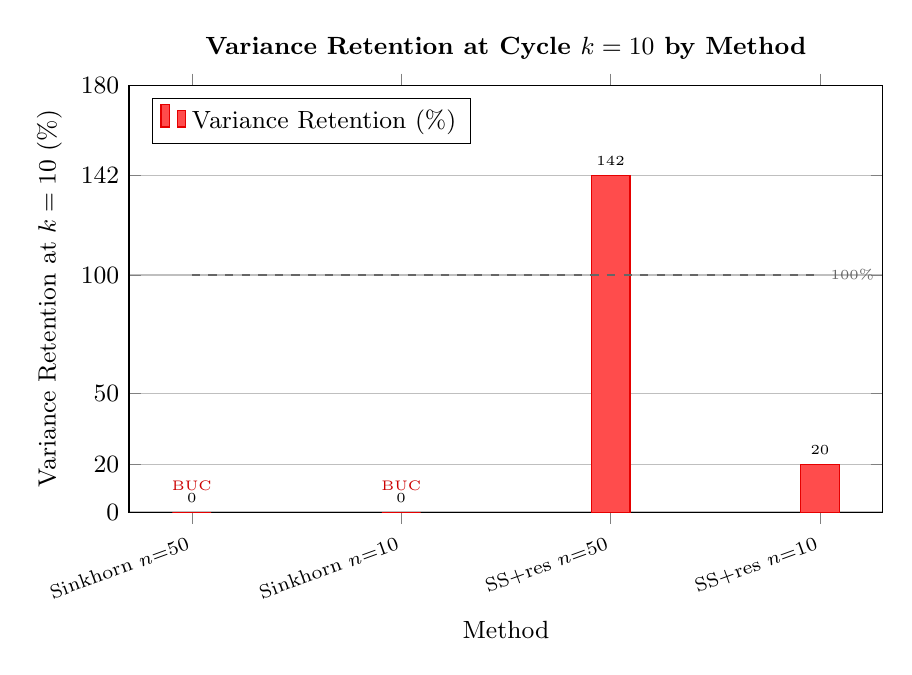
\begin{tikzpicture}
  \begin{axis}[
    width=0.92\linewidth,
    height=7.0cm,
    ybar,
    bar width=14pt,
    xlabel={Method},
    ylabel={Variance Retention at $k=10$ (\%)},
    symbolic x coords={
      {Sinkhorn $n{=}50$},
      {Sinkhorn $n{=}10$},
      {SS+res $n{=}50$},
      {SS+res $n{=}10$}
    },
    xtick=data,
    xticklabel style={
      font=\scriptsize,
      rotate=20,
      anchor=north east,
    },
    ymin=0,
    ymax=180,
    ytick={0,20,50,100,142,180},
    yticklabels={0,20,50,100,142,180},
    tick label style={font=\small},
    label style={font=\small},
    title style={font=\small\bfseries},
    title={Variance Retention at Cycle $k=10$ by Method},
    ymajorgrids,
    grid style={line width=0.3pt, draw=gray!30},
    major grid style={line width=0.6pt, draw=gray!50},
    nodes near coords,
    nodes near coords style={
      font=\tiny,
      /pgf/number format/.cd, fixed, precision=0,
    },
    legend pos=north west,
    legend style={font=\small},
    clip=false,
  ]

  %% Data: variance retention at k=10
  \addplot[
    fill=red!70,
    draw=red!90!black,
  ] coordinates {
    ({Sinkhorn $n{=}50$}, 0)
	    ({Sinkhorn $n{=}10$}, 0)
	    ({SS+res $n{=}50$},  142)
	    ({SS+res $n{=}10$},   20)
  };
  \addlegendentry{Variance Retention (\%)}

  %% Reference line at 100% (initial variance)
  \draw[dashed, black!60, line width=1pt]
	    (axis cs:{Sinkhorn $n{=}50$},100) -- (axis cs:{SS+res $n{=}10$},100)
    node[right, font=\tiny, black!60] {100\%};

  %% Annotation: BUC
  \node[font=\tiny, red!80!black, anchor=south] at (axis cs:{Sinkhorn $n{=}50$},5)
    {BUC};
  \node[font=\tiny, red!80!black, anchor=south] at (axis cs:{Sinkhorn $n{=}10$},5)
    {BUC};

	  \end{axis}
\end{tikzpicture}
 inside a figure environment
%
% Shows variance retention at cycle k=10 for source-backed discrete methods.

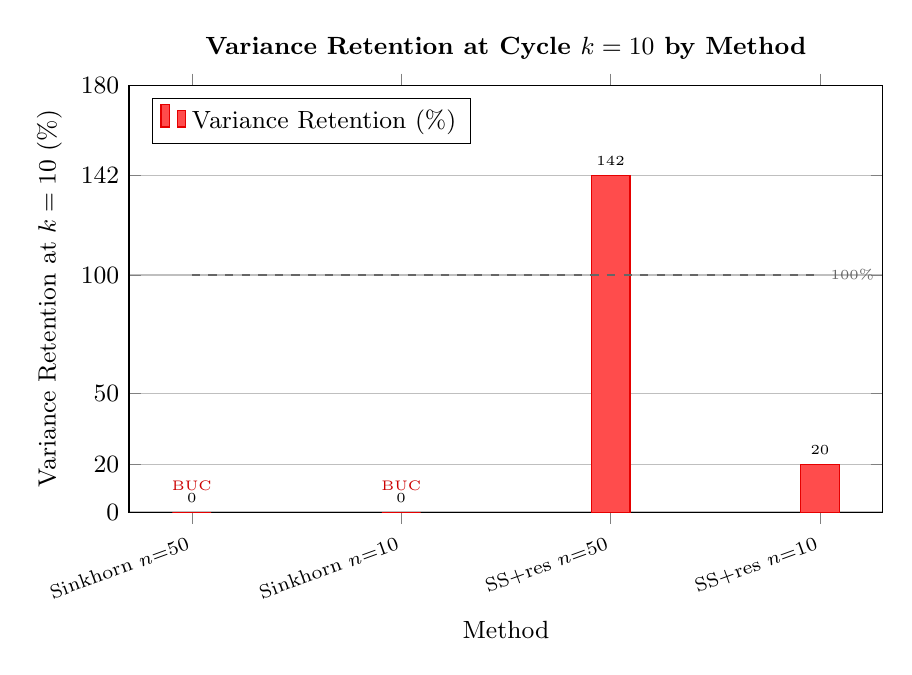
\begin{tikzpicture}
  \begin{axis}[
    width=0.92\linewidth,
    height=7.0cm,
    ybar,
    bar width=14pt,
    xlabel={Method},
    ylabel={Variance Retention at $k=10$ (\%)},
    symbolic x coords={
      {Sinkhorn $n{=}50$},
      {Sinkhorn $n{=}10$},
      {SS+res $n{=}50$},
      {SS+res $n{=}10$}
    },
    xtick=data,
    xticklabel style={
      font=\scriptsize,
      rotate=20,
      anchor=north east,
    },
    ymin=0,
    ymax=180,
    ytick={0,20,50,100,142,180},
    yticklabels={0,20,50,100,142,180},
    tick label style={font=\small},
    label style={font=\small},
    title style={font=\small\bfseries},
    title={Variance Retention at Cycle $k=10$ by Method},
    ymajorgrids,
    grid style={line width=0.3pt, draw=gray!30},
    major grid style={line width=0.6pt, draw=gray!50},
    nodes near coords,
    nodes near coords style={
      font=\tiny,
      /pgf/number format/.cd, fixed, precision=0,
    },
    legend pos=north west,
    legend style={font=\small},
    clip=false,
  ]

  %% Data: variance retention at k=10
  \addplot[
    fill=red!70,
    draw=red!90!black,
  ] coordinates {
    ({Sinkhorn $n{=}50$}, 0)
	    ({Sinkhorn $n{=}10$}, 0)
	    ({SS+res $n{=}50$},  142)
	    ({SS+res $n{=}10$},   20)
  };
  \addlegendentry{Variance Retention (\%)}

  %% Reference line at 100% (initial variance)
  \draw[dashed, black!60, line width=1pt]
	    (axis cs:{Sinkhorn $n{=}50$},100) -- (axis cs:{SS+res $n{=}10$},100)
    node[right, font=\tiny, black!60] {100\%};

  %% Annotation: BUC
  \node[font=\tiny, red!80!black, anchor=south] at (axis cs:{Sinkhorn $n{=}50$},5)
    {BUC};
  \node[font=\tiny, red!80!black, anchor=south] at (axis cs:{Sinkhorn $n{=}10$},5)
    {BUC};

	  \end{axis}
\end{tikzpicture}
 inside a figure environment
%
% Shows variance retention at cycle k=10 for source-backed discrete methods.

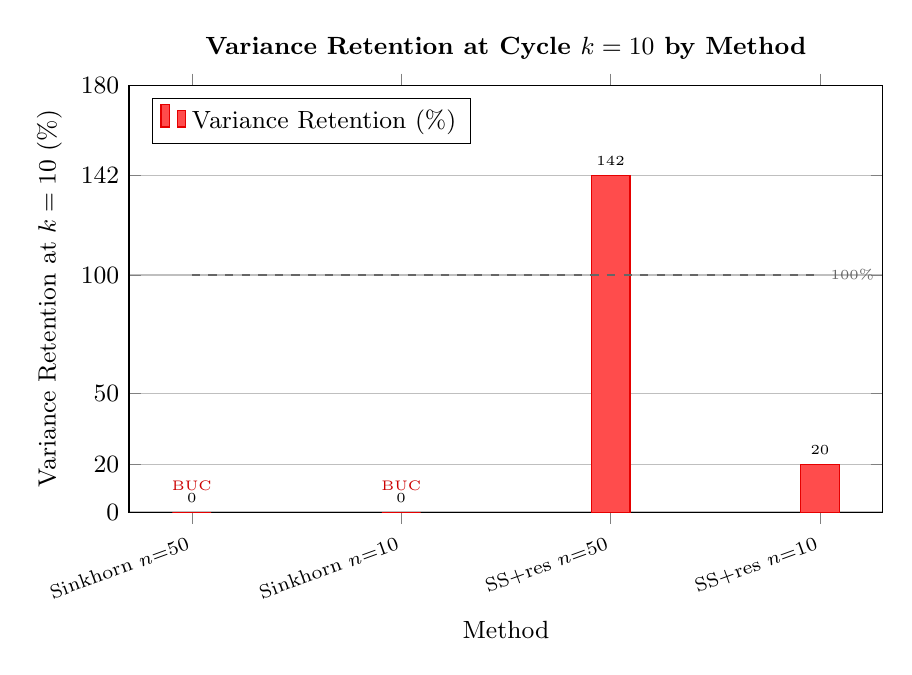
\begin{tikzpicture}
  \begin{axis}[
    width=0.92\linewidth,
    height=7.0cm,
    ybar,
    bar width=14pt,
    xlabel={Method},
    ylabel={Variance Retention at $k=10$ (\%)},
    symbolic x coords={
      {Sinkhorn $n{=}50$},
      {Sinkhorn $n{=}10$},
      {SS+res $n{=}50$},
      {SS+res $n{=}10$}
    },
    xtick=data,
    xticklabel style={
      font=\scriptsize,
      rotate=20,
      anchor=north east,
    },
    ymin=0,
    ymax=180,
    ytick={0,20,50,100,142,180},
    yticklabels={0,20,50,100,142,180},
    tick label style={font=\small},
    label style={font=\small},
    title style={font=\small\bfseries},
    title={Variance Retention at Cycle $k=10$ by Method},
    ymajorgrids,
    grid style={line width=0.3pt, draw=gray!30},
    major grid style={line width=0.6pt, draw=gray!50},
    nodes near coords,
    nodes near coords style={
      font=\tiny,
      /pgf/number format/.cd, fixed, precision=0,
    },
    legend pos=north west,
    legend style={font=\small},
    clip=false,
  ]

  %% Data: variance retention at k=10
  \addplot[
    fill=red!70,
    draw=red!90!black,
  ] coordinates {
    ({Sinkhorn $n{=}50$}, 0)
	    ({Sinkhorn $n{=}10$}, 0)
	    ({SS+res $n{=}50$},  142)
	    ({SS+res $n{=}10$},   20)
  };
  \addlegendentry{Variance Retention (\%)}

  %% Reference line at 100% (initial variance)
  \draw[dashed, black!60, line width=1pt]
	    (axis cs:{Sinkhorn $n{=}50$},100) -- (axis cs:{SS+res $n{=}10$},100)
    node[right, font=\tiny, black!60] {100\%};

  %% Annotation: BUC
  \node[font=\tiny, red!80!black, anchor=south] at (axis cs:{Sinkhorn $n{=}50$},5)
    {BUC};
  \node[font=\tiny, red!80!black, anchor=south] at (axis cs:{Sinkhorn $n{=}10$},5)
    {BUC};

	  \end{axis}
\end{tikzpicture}
 inside a figure environment
%
% Shows variance retention at cycle k=10 for source-backed discrete methods.

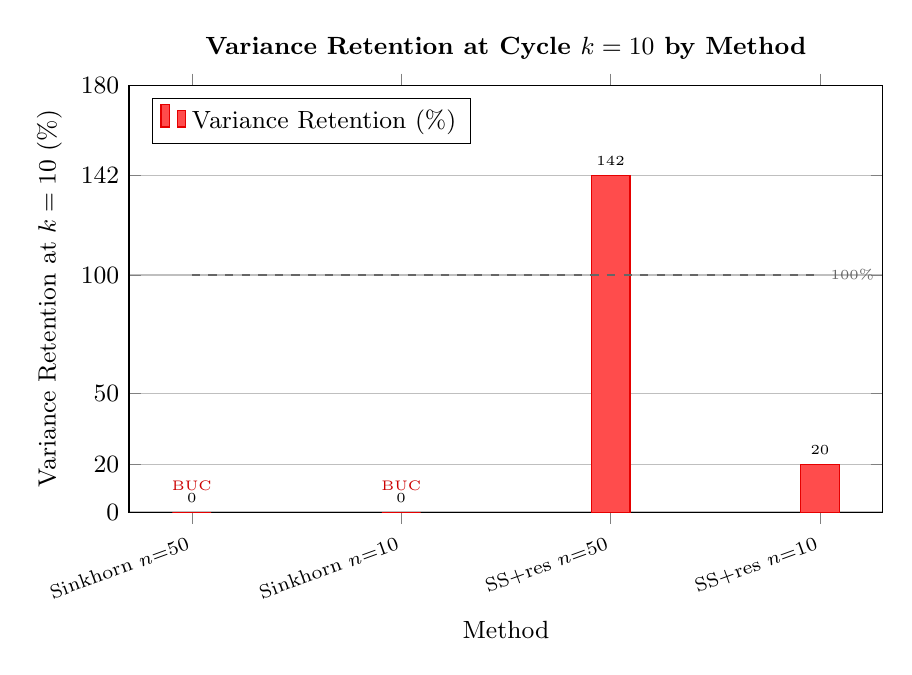
\begin{tikzpicture}
  \begin{axis}[
    width=0.92\linewidth,
    height=7.0cm,
    ybar,
    bar width=14pt,
    xlabel={Method},
    ylabel={Variance Retention at $k=10$ (\%)},
    symbolic x coords={
      {Sinkhorn $n{=}50$},
      {Sinkhorn $n{=}10$},
      {SS+res $n{=}50$},
      {SS+res $n{=}10$}
    },
    xtick=data,
    xticklabel style={
      font=\scriptsize,
      rotate=20,
      anchor=north east,
    },
    ymin=0,
    ymax=180,
    ytick={0,20,50,100,142,180},
    yticklabels={0,20,50,100,142,180},
    tick label style={font=\small},
    label style={font=\small},
    title style={font=\small\bfseries},
    title={Variance Retention at Cycle $k=10$ by Method},
    ymajorgrids,
    grid style={line width=0.3pt, draw=gray!30},
    major grid style={line width=0.6pt, draw=gray!50},
    nodes near coords,
    nodes near coords style={
      font=\tiny,
      /pgf/number format/.cd, fixed, precision=0,
    },
    legend pos=north west,
    legend style={font=\small},
    clip=false,
  ]

  %% Data: variance retention at k=10
  \addplot[
    fill=red!70,
    draw=red!90!black,
  ] coordinates {
    ({Sinkhorn $n{=}50$}, 0)
	    ({Sinkhorn $n{=}10$}, 0)
	    ({SS+res $n{=}50$},  142)
	    ({SS+res $n{=}10$},   20)
  };
  \addlegendentry{Variance Retention (\%)}

  %% Reference line at 100% (initial variance)
  \draw[dashed, black!60, line width=1pt]
	    (axis cs:{Sinkhorn $n{=}50$},100) -- (axis cs:{SS+res $n{=}10$},100)
    node[right, font=\tiny, black!60] {100\%};

  %% Annotation: BUC
  \node[font=\tiny, red!80!black, anchor=south] at (axis cs:{Sinkhorn $n{=}50$},5)
    {BUC};
  \node[font=\tiny, red!80!black, anchor=south] at (axis cs:{Sinkhorn $n{=}10$},5)
    {BUC};

	  \end{axis}
\end{tikzpicture}
